\documentclass [a4paper, 11pt, titlepage] {article}

\usepackage[english]{babel}
\usepackage[ansinew]{inputenc}
\usepackage{amsmath,amssymb,amsfonts}
\usepackage{verbatim}
\usepackage{graphicx}
\usepackage{algorithm,algorithmic}
\usepackage{pgfplots}
\pgfplotsset{compat=1.16}
\usepgfplotslibrary{statistics}
\hyphenation{desirable finally sta-ti-sti-cal-ly basic tailored}
\date{\today}

%BEGIN Changing sizes of captions:
\newcommand{\captionfonts}{\footnotesize}

\makeatletter  % Allow the use of @ in command names
\long\def\@makecaption#1#2{%
  \vskip\abovecaptionskip
  \sbox\@tempboxa{{\captionfonts #1: #2}}%
  \ifdim \wd\@tempboxa >\hsize
    {\captionfonts #1: #2\par}
  \else
    \hbox to\hsize{\hfil\box\@tempboxa\hfil}%
  \fi
  \vskip\belowcaptionskip}
\makeatother   % Cancel the effect of \makeatletter
%END Changing sizes of captions.


\begin{document}

\setlength{\parindent}{4mm}
\renewcommand{\algorithmiccomment}[1]{//#1}

\begin{titlepage}
  \begin{center}
    \vspace*{\stretch{1}}
    \noindent\rule{\linewidth}{1mm}\\[4mm]
      {\sffamily\bfseries \Huge Bus Transit Route Network Design Problem}\\[1mm]
	{\sffamily\bfseries \Large
        Project Final Report}\\[0mm]
      {\sffamily\bfseries \Large
        EMU676 Optimization Models and Algorithms in Transportation and Distribution}\\[0mm]
    \noindent\rule{\linewidth}{1mm}\\[30mm]
    \large Fatih Alper Vural -- ``N25123161'' \\

    \vspace*{\stretch{3}}

    \large \today \\[6mm]
    Hacettepe University
  \end{center}
\end{titlepage}

\newpage
\pagenumbering{roman}
\tableofcontents
\newpage
\pagenumbering{arabic}

% ============================ INTRODUCTION ============================
\section{Introduction}
\label{introduction}

The Bus Transit Route Network Design Problem (BTRNDP) seeks the set of bus
routes and their service frequencies that best serve a given travel demand while
balancing the conflicting interests of passengers and operators. The problem is
NP--hard: the number of candidate route configurations grows exponentially with
the size of the network, so exact methods are intractable for realistic
instances and metaheuristics are the standard solution approach. This report
implements and evaluates the Simulated Annealing (SA) framework of Fan and
Machemehl \cite{fan2006}, in which the problem is modelled at the
distribution--node level, unsatisfied demand enters the objective directly, and
route frequencies are determined endogenously through a transit--assignment
model.

The remainder of this report is organised as follows. In section
\ref{problem_formulation} the BTRNDP is defined and its mathematical model is
stated. In section \ref{algorithm} the SA metaheuristic is introduced, together
with the candidate route generator, the network analysis (evaluation) procedure,
the solution encoding and neighbourhood operator, and the constraint--handling
scheme. Section \ref{sec:results} describes the test instance, the parameter
tuning, and the computational results, including a statistical comparison of SA
against a Genetic Algorithm (GA) baseline. We conclude the report in section
\ref{sec:conclusion}. The complete source code, input data, and result files are
available in the public repository referenced in section \ref{sec:repo}.

% ========================= PROBLEM FORMULATION =========================
\section{Problem Formulation}
\label{problem_formulation}

\subsection{Problem Description}
The transportation network is modelled as a directed graph $G=(N,A)$, where $N$
is a set of nodes (each representing a demand centroid as well as a physical
junction) and $A$ a set of directed arcs. A \emph{route} is a sequence of nodes
in which each consecutive pair is connected by an arc; the \emph{headway} of a
route is the inter--arrival time of its buses and the \emph{frequency} is its
reciprocal. Travel demand $d_{ij}$ between centroids $i$ and $j$ may be served
\emph{directly} (a single route connects $i$ and $j$), via a \emph{transfer}
(two routes sharing a common node), or it may be left \emph{unsatisfied}.

The BTRNDP simultaneously minimises three competing cost components:
(i) passenger user cost (in--vehicle time, waiting time, and transfer
penalties); (ii) operator cost, proportional to the total vehicle--hours
deployed; and (iii) unsatisfied--demand cost, which penalises O--D pairs for
which no feasible path exists. Weights $C_1$, $C_2$, $C_3$ balance the three
components. As Fan and Machemehl \cite{fan2006} observe, omitting the third
component would render the trivial ``no service'' solution optimal, so its
inclusion is essential.

\subsection{Mathematical Model}
The BTRNDP is formulated as a multiobjective nonlinear mixed--integer program
\cite{fan2006}. The objective minimises the weighted sum of user cost, operator
cost, and unsatisfied--demand cost:
\begin{alignat}{2}
  \min~ z = ~& C_1 \Bigg[ \sum_{i\in N}\sum_{j\in N}\sum_{r_m\in DR_{ij}}
     d^{r_m}_{ij}\,t^{r_m}_{ij}
     + \sum_{i\in N}\sum_{j\in N}\sum_{tr\in TR_{ij}}
     d^{tr}_{ij}\,t^{tr}_{ij} \Bigg] \notag \\
   & + C_2 \, \frac{C_v}{C_m}\,O_v \sum_{m=1}^{M}\frac{T_{r_m}}{h_{r_m}}
     \notag \\
   & + C_3 \, \frac{C_d}{C_m}\Bigg[ \sum_{i,j\in N} d_{ij}
     - \sum_{i,j\in N}\sum_{r_m\in DR_{ij}} d^{r_m}_{ij}
     - \sum_{i,j\in N}\sum_{tr\in TR_{ij}} d^{tr}_{ij} \Bigg]
     \label{eq:obj}
\end{alignat}
subject to
\begin{alignat}{2}
  & h_{\min} \leq h_{r_m} \leq h_{\max}, & \quad & \forall\, r_m \in R
     \label{eq:c1}\\
  & L_{r_m} = \frac{Q^{\max}_{r_m}\,h_{r_m}}{P} \leq L_{\max}, & \quad &
     \forall\, r_m \in R \label{eq:c2}\\
  & \sum_{m=1}^{M}\frac{T_{r_m}}{h_{r_m}} \leq W & & \label{eq:c3}\\
  & D_{\min} \leq D_{r_m} \leq D_{\max}, & \quad & \forall\, r_m \in R
     \label{eq:c4}\\
  & M \leq R_{\max} & & \label{eq:c5}\\
  & \sum_{i}\sum_{j}\!\Big( \!\sum_{r_m\in DR_{ij}}\! d^{r_m}_{ij}
     + \!\sum_{tr\in TR_{ij}}\! d^{tr}_{ij}\Big)
     \geq (1-U_{\max})\!\sum_{i,j\in N}\! d_{ij} & & \label{eq:c6}\\
  & M,\,h_{r_m},\,Q^{\max}_{r_m},\,d^{r_m}_{ij},\,d^{tr}_{ij}
     \in \mathbb{Z}^{+}. & & \label{eq:c7}
\end{alignat}

Here $M$ is the number of routes, $r_m$ the $m$--th route, $D_{r_m}$ its length,
$T_{r_m}$ its round--trip time, $h_{r_m}$ its headway, $L_{r_m}$ its load factor,
and $Q^{\max}_{r_m}$ the maximum passenger flow on its critical link; $DR_{ij}$
and $TR_{ij}$ are the sets of direct routes and transfer paths serving $(i,j)$.
Constraint \eqref{eq:c1} enforces policy headways; \eqref{eq:c2} prevents
overloading the critical link; \eqref{eq:c3} limits deployed buses to the fleet
$W$; \eqref{eq:c4} bounds route length; \eqref{eq:c5} caps the number of routes;
\eqref{eq:c6} guarantees the served fraction of demand; and \eqref{eq:c7}
enforces integrality. The baseline weights are $(C_1,C_2,C_3)=(0.4,0.4,0.2)$.

% ===================== DESCRIPTION OF THE ALGORITHM =====================
\section{Description of the Metaheuristic Algorithm}
\label{algorithm}

The solution framework comprises three integrated components: (1) an Initial
Candidate Route Set Generation Procedure (ICRSGP) that precomputes a pool of
feasible candidate routes; (2) a Network Analysis Procedure (NAP) that evaluates
any route set by assigning demand and determining frequencies; and (3) a
Simulated Annealing (SA) loop that searches the candidate pool for the best
route set. Simulated Annealing \cite{eglese1990} is a local--search
metaheuristic that escapes local optima by occasionally accepting worse
solutions with a probability that decreases as a ``temperature'' parameter is
cooled.

\subsection{The Algorithm}
The top--level procedure is given in Algorithm \ref{alg:sa}. An outer loop grows
the route--set size $n$ from $1$ to $R_{\max}$ (line 3); for each size an inner
SA search is run on solutions of that fixed size. A candidate neighbour is
generated by the \emph{swap} operator (line 8), and accepted if it improves the
objective or, otherwise, with the Metropolis probability $e^{-\Delta z/T}$
(line 13). The temperature $T$ is reduced geometrically by the factor $\alpha$
every $K$ iterations (line 17), and the search stops after $G_{\max}$ cooling
steps. The best feasible solution encountered across all sizes is returned.

\begin{algorithm}
  \caption{SA Framework for the BTRNDP} \label{alg:sa}
  \begin{algorithmic}[1]
    \STATE $Pool \leftarrow$ ICRSGP()
    \STATE $Best \leftarrow \emptyset$
    \FOR{$n = 1$ to $R_{\max}$}
      \STATE $S \leftarrow$ RandomSolution($Pool$, $n$);~~ $T \leftarrow T_0$;~~ $g \leftarrow 0$;~~ $k \leftarrow 0$
      \WHILE{$g < G_{\max}$}
        \STATE evaluate $z(S)$ via NAP($S$)
        \STATE $S' \leftarrow$ Neighbour($S$);~~ evaluate $z(S')$
        \STATE $\Delta z \leftarrow z(S') - z(S)$
        \IF{$\Delta z < 0$}
          \STATE $S \leftarrow S'$
          \IF{$z(S') < z(Best)$} \STATE $Best \leftarrow S'$ \ENDIF
        \ELSE
          \STATE draw $p \sim U[0,1]$
          \IF{$p < e^{-\Delta z / T}$} \STATE $S \leftarrow S'$ \ENDIF
        \ENDIF
        \STATE $k \leftarrow k + 1$
        \IF{$k \geq K$} \STATE $T \leftarrow \alpha T$;~~ $k \leftarrow 0$;~~ $g \leftarrow g + 1$ \ENDIF
      \ENDWHILE
    \ENDFOR
    \STATE \textbf{return} $Best$
  \end{algorithmic}
\end{algorithm}

\subsection{Initial Candidate Route Set Generation}
The ICRSGP, shown in Algorithm \ref{alg:icrsgp}, enumerates feasible candidate
routes once, before optimisation. For every centroid pair $(i,j)$, Dijkstra's
algorithm \cite{ahuja1993} produces the shortest path and Yen's algorithm
\cite{yen1971} produces up to $k=6$ loopless alternatives. A generated path is
retained only if its length satisfies $D_{\min} \leq D_{r_m} \leq D_{\max}$, so
that route--length feasibility \eqref{eq:c4} holds for every pool member by
construction. Each route and its reverse are canonicalised to a single
representative to avoid duplicate work. On the test instance this produces a
pool of $569$ feasible candidate routes in $0.03$ seconds.

\begin{algorithm}
  \caption{ICRSGP} \label{alg:icrsgp}
  \begin{algorithmic}[1]
    \STATE $Pool \leftarrow \emptyset$
    \FOR{every centroid pair $(i,j)$}
      \STATE compute shortest path (Dijkstra); generate $k$ alternatives (Yen)
      \FOR{each generated path $P$}
        \IF{$D_{\min} \leq \mathrm{length}(P) \leq D_{\max}$}
          \STATE canonicalise $P$ (merge with its reverse); add $P$ to $Pool$
        \ENDIF
      \ENDFOR
    \ENDFOR
    \STATE \textbf{return} $Pool$
  \end{algorithmic}
\end{algorithm}

\subsection{Network Analysis Procedure}
Given a route set, the NAP returns the objective value \eqref{eq:obj} together
with feasibility information. It performs a lexicographic transit assignment
followed by endogenous frequency setting, iterated to convergence (three
iterations in the implementation):
\begin{itemize}
\item \emph{Priority 1 -- direct service.} If one or more routes serve $(i,j)$
directly, the demand $d_{ij}$ is split among them inversely proportional to
in--vehicle travel time, so that faster routes attract more passengers.
\item \emph{Priority 2 -- one transfer.} If no direct route exists, demand is
routed over a pair of routes sharing a common node, with a transfer penalty of
five equivalent minutes added to the travel time.
\item \emph{Unsatisfied.} Demand with no path of either kind is recorded as
unsatisfied and penalised through the third term of \eqref{eq:obj}.
\end{itemize}
After each assignment pass, the headway of each route is recomputed from the
flow $q_{\max}$ on its critical link using the load--factor relation
$h \leq 60\,L_{\max}P/q_{\max}$, clamped to $[h_{\min},h_{\max}]$, and the demand
is reassigned. For efficiency the assignment logic is implemented as a single
reusable routine, and each route precomputes its segment times, cumulative
times, and node positions; this brings a full SA run to roughly $3.4$ seconds.

\subsection{Solution Encoding and Neighbourhood Operator}
A solution is encoded as a \emph{set of integer indices} into the candidate
pool, of cardinality $n \leq R_{\max}$. This compact encoding makes the SA loop
independent of route geometry and guarantees length feasibility by construction.
The neighbourhood operator Neighbour($S$) performs a single--route \emph{swap}:
one index in $S$ is replaced by a uniformly random index from the pool that is
not already present. This move is inexpensive, preserves the solution size $n$,
and induces a connected search space, which is the standard requirement for the
convergence behaviour of SA.

\subsection{Constraint Handling}
Constraints \eqref{eq:c4} and \eqref{eq:c5} are enforced structurally by the
encoding. The remaining constraints -- fleet size \eqref{eq:c3}, unsatisfied
demand \eqref{eq:c6}, and load factor \eqref{eq:c2} -- are handled with a
\emph{fixed--plus--marginal} penalty added to \eqref{eq:obj}. For each violated
constraint a large fixed term (5000) plus a marginal term proportional to the
amount of violation is added. The large fixed component guarantees that any
feasible solution dominates any infeasible one, while the marginal component
gives the search a usable gradient out of the infeasible region. This design
proved necessary because the test demand is deliberately heavy relative to the
fleet, so most random starts are infeasible.

\subsection{Genetic Algorithm Baseline}
For comparison, a Genetic Algorithm (GA) \cite{pattnaik1998} was implemented over
the same encoding. A chromosome is a set of at most $R_{\max}$ route indices;
selection is by binary tournament; crossover takes the union of two parents and
trims it to a feasible size; and mutation swaps one route index. The GA uses a
population of $24$ for $40$ generations and is evaluated with the identical NAP,
so that the comparison is fair.

% ============================== RESULTS ==============================
\section{Results}
\label{sec:results}

\subsection{Test Instance}
Because the exact node coordinates and demand matrix of the published
Mandl--scale network in \cite{fan2006} are not available for verbatim
reproduction, a fully--specified benchmark of comparable scale was generated
deterministically (without a random seed) and is shipped with the code so that
all results are exactly reproducible. The instance has $15$ nodes and $23$
undirected links ($46$ directed arcs); travel time is $2$ min/km (a $30$ km/h
operating speed). Demand follows a gravity model
$d_{ij}=\mathrm{round}(K\,w_i w_j / \mathrm{dist}_{ij})$ with node weights $w$
and calibration constant $K=38$; flows below $5$ pass./h are dropped. The result
is $102$ O--D pairs with positive demand and a total demand of $7172$ pass./h.
The operational parameters are summarised in Table \ref{tab:params}.

\begin{table}[!htb]
  \centering
  \begin{tabular}{|l|c|l|c|}
    \hline
    Parameter & Value & Parameter & Value \\
    \hline
    Max.\ routes $R_{\max}$       & 8        & Bus capacity $P$       & 90 \\
    Max.\ unsatisfied $U_{\max}$  & 0.15     & Fleet size $W$         & 58 \\
    Route length $[D_{\min},D_{\max}]$ & $[3,30]$ km & Load factor $L_{\max}$ & 1.0 \\
    Headway $[h_{\min},h_{\max}]$ & $[5,30]$ min & Weights $(C_1,C_2,C_3)$ & $(0.4,0.4,0.2)$ \\
    \hline
  \end{tabular}
  \caption{Operational parameters of the test instance.}
  \label{tab:params}
\end{table}

\subsection{Parameter Tuning}
The SA has four parameters: the initial temperature $T_0$, the cooling
coefficient $\alpha$, the maximum number of cooling steps $G_{\max}$, and the
repetition counter $K$. Following the tuning protocol of \cite{fan2006}, a grid
over $T_0 \in \{500,1000,2000,5000\}$ and $\alpha \in \{0.5,0.6,0.7,0.9\}$ was
evaluated, with three replications per cell using a shortened schedule
($G_{\max}=15$, $K=8$). The selection criterion is the lowest mean objective
combined with the smallest standard deviation. Table \ref{tab:tuning} reports
the mean (and standard deviation) of $z$ for each cell.

\begin{table}[!htb]
  \centering
  \begin{tabular}{|r|c|c|c|c|}
    \hline
    $T_0 \backslash \alpha$ & 0.5 & 0.6 & 0.7 & 0.9 \\
    \hline
    500  & 50859 (490)  & 50859 (490)  & 50859 (490)  & 51526 (1312) \\
    1000 & 50482 (588)  & 50795 (466)  & 50795 (466)  & 51959 (1908) \\
    2000 & 50632 (323)  & \textbf{50462 (869)} & 51258 (1058) & 51784 (2372) \\
    5000 & 48934 (2025) & 52178 (1711) & 52426 (989)  & 50908 (1331) \\
    \hline
  \end{tabular}
  \caption{Parameter--tuning grid: mean $z$ with standard deviation in
  parentheses, three runs per cell. The single lowest mean
  ($T_0{=}5000,\alpha{=}0.5$) is unstable ($\delta=2025$); the most stable strong
  cell (in bold) is $T_0{=}2000,\alpha{=}0.6$.}
  \label{tab:tuning}
\end{table}

The grid confirms the parameter region reported by Fan and Machemehl
\cite{fan2006}. Although the single lowest mean occurs at
$T_0{=}5000,\alpha{=}0.5$, that cell has very high variance ($\delta=2025$).
Applying the joint mean--variance criterion, the configuration
$T_0{=}2000,\alpha{=}0.6$ gives the best trade--off (mean $50462$, $\delta=869$)
and matches the optimal values of \cite{fan2006}; together with $G_{\max}=20$
and $K=10$ it is adopted for all final experiments.

\subsection{Computational Results}
Each method was run for $20$ independent replications with distinct seeds. The
key performance measure, following \cite{fan2006}, is the \emph{gap} between the
best--known solution and the mean performance of the metaheuristic,
\begin{equation}
  gap = 100 \cdot \frac{(Mean - Best)}{Best}, \nonumber
\end{equation}
where $Best$ is the lowest objective found across all SA and GA runs ($z^{*} =
45361.1$), used as the reference because no published optimum exists for the
generated instance. Table \ref{tab:summary} reports the aggregate performance
and Table \ref{tab:perrun} lists the per--run objectives and gaps.

\begin{table}[!htb]
  \centering
  \begin{tabular}{|l|r|r|r|r|r|r|}
    \hline
    Method & Mean $z$ & Std $z$ & Min $z$ & Max $z$ & Gap (\%) & Time (s) \\
    \hline
    SA & 48841.7 & 2405.2 & 45361.1 & 52989.5 & 7.67  & 3.37 \\
    GA & 52940.7 & 2996.2 & 45855.7 & 58148.6 & 16.71 & 2.19 \\
    \hline
  \end{tabular}
  \caption{Aggregate performance over 20 runs
  ($T_0{=}2000$, $\alpha{=}0.6$, $G_{\max}{=}20$, $K{=}10$).}
  \label{tab:summary}
\end{table}

SA attains a mean objective $7.7\%$ lower than the GA and a markedly tighter
distribution. Of the $20$ SA runs, $8$ finished within $5\%$ of the best--known
solution, against only $1$ for the GA. The higher mean CPU time of SA
($3.37$ s versus $2.19$ s) reflects the iterative frequency--update loop inside
the NAP; both methods remain well within interactive time on this instance.

\begin{table}[!htb]
  \footnotesize
  \centering
  \begin{tabular}{|r|r|r|r|r||r|r|r|r|r|}
    \hline
    Run & SA $z$ & gap\% & GA $z$ & gap\% & Run & SA $z$ & gap\% & GA $z$ & gap\% \\
    \hline
    0 & 45865.1 & 1.11  & 50575.9 & 11.5 & 10 & 46523.8 & 2.56  & 50769.7 & 11.9 \\
    1 & 49779.1 & 9.74  & 45855.7 & 1.1  & 11 & 51738.4 & 14.06 & 50385.1 & 11.1 \\
    2 & 51410.6 & 13.34 & 53768.3 & 18.5 & 12 & 45361.1 & 0.00  & 49570.6 & 9.3  \\
    3 & 47418.5 & 4.54  & 51146.1 & 12.8 & 13 & 50817.7 & 12.03 & 53988.3 & 19.0 \\
    4 & 48962.2 & 7.94  & 54969.3 & 21.2 & 14 & 46783.4 & 3.13  & 51201.8 & 12.9 \\
    5 & 48159.4 & 6.17  & 53423.1 & 17.8 & 15 & 46411.3 & 2.31  & 52050.2 & 14.7 \\
    6 & 51364.6 & 13.23 & 58148.6 & 28.2 & 16 & 45520.6 & 0.35  & 56075.9 & 23.6 \\
    7 & 51089.7 & 12.63 & 51763.1 & 14.1 & 17 & 49364.1 & 8.82  & 57414.9 & 26.6 \\
    8 & 50580.4 & 11.51 & 50563.4 & 11.5 & 18 & 50944.5 & 12.31 & 54944.0 & 21.1 \\
    9 & 45749.9 & 0.86  & 56059.5 & 23.6 & 19 & 52989.6 & 16.82 & 56139.6 & 23.8 \\
    \hline
  \end{tabular}
  \caption{Per--run objective values and gaps to the best--known solution
  ($z^{*}=45361.1$) for all 20 replications of each method.}
  \label{tab:perrun}
\end{table}

Figure \ref{fig:conv} shows the convergence of the incumbent objective for the
best SA run. The incumbent drops rapidly from a heavily penalised infeasible
start while the temperature is high, then refines locally as $T \to 0$,
finishing at the feasible optimum $z=45361.1$. Figure \ref{fig:box} contrasts
the objective distributions of the two methods over the $20$ runs.

\begin{figure}[!htb]
  \centering
  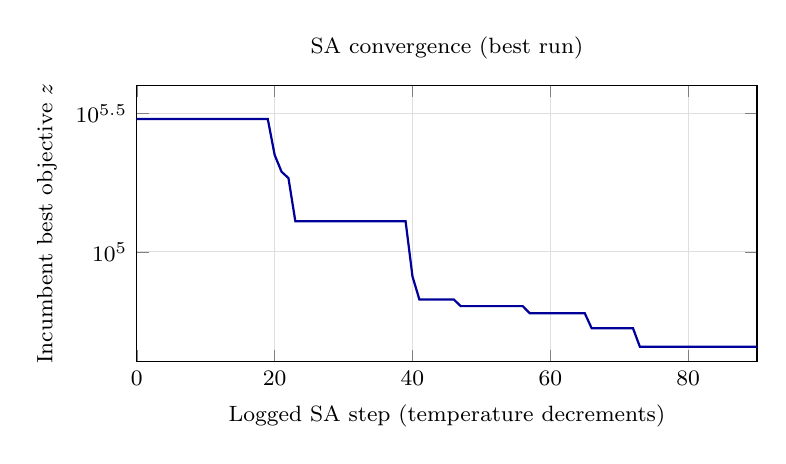
\begin{tikzpicture}
    \begin{axis}[
        width=0.78\textwidth, height=0.42\textwidth,
        ymode=log,
        xlabel={Logged SA step (temperature decrements)},
        ylabel={Incumbent best objective $z$},
        xmin=0, xmax=90,
        ymin=40000, ymax=400000,
        grid=both, grid style={gray!25},
        tick label style={font=\footnotesize},
        label style={font=\footnotesize},
        title style={font=\footnotesize}, title={SA convergence (best run)},
      ]
      \addplot[blue!60!black, thick, mark=none] coordinates {
        (0,302195.5) (1,302195.5) (2,302195.5) (3,302195.5) (4,302195.5)
        (5,302195.5) (6,302195.5) (7,302195.5) (8,302195.5) (9,302195.5)
        (10,302195.5) (11,302195.5) (12,302195.5) (13,302195.5) (14,302195.5)
        (15,302195.5) (16,302195.5) (17,302195.5) (18,302195.5) (19,302195.5)
        (20,224020.7) (21,194865.4) (22,184917.0) (23,128974.6) (24,128974.6)
        (25,128974.6) (26,128974.6) (27,128974.6) (28,128974.6) (29,128974.6)
        (30,128974.6) (31,128974.6) (32,128974.6) (33,128974.6) (34,128974.6)
        (35,128974.6) (36,128974.6) (37,128974.6) (38,128974.6) (39,128974.6)
        (40,81457.0) (41,67241.1) (42,67241.1) (43,67241.1) (44,67241.1)
        (45,67241.1) (46,67241.1) (47,63629.3) (48,63629.3) (49,63629.3)
        (50,63629.3) (51,63629.3) (52,63629.3) (53,63629.3) (54,63629.3)
        (55,63629.3) (56,63629.3) (57,60015.1) (58,60015.1) (59,60015.1)
        (60,60015.1) (61,60015.1) (62,60015.1) (63,60015.1) (64,60015.1)
        (65,60015.1) (66,52927.8) (67,52927.8) (68,52927.8) (69,52927.8)
        (70,52927.8) (71,52927.8) (72,52927.8) (73,45361.1) (74,45361.1)
        (75,45361.1) (80,45361.1) (85,45361.1) (90,45361.1)
      };
    \end{axis}
  \end{tikzpicture}
  \caption{Convergence of the incumbent objective for the best SA run
  (logarithmic vertical axis).}
  \label{fig:conv}
\end{figure}

\begin{figure}[!htb]
  \centering
  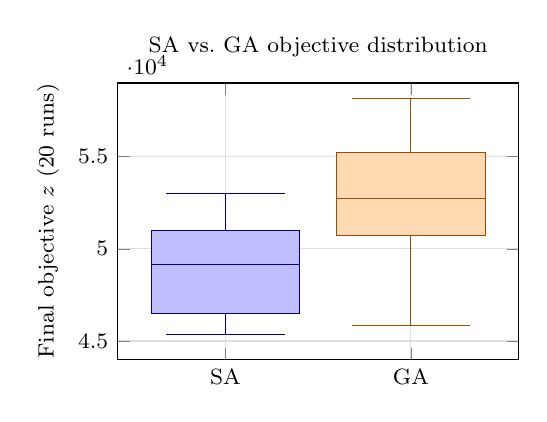
\begin{tikzpicture}
    \begin{axis}[
        width=0.55\textwidth, height=0.42\textwidth,
        ylabel={Final objective $z$ (20 runs)},
        boxplot/draw direction=y,
        xtick={1,2}, xticklabels={SA, GA},
        ymin=44000, ymax=59000,
        grid=major, grid style={gray!25},
        tick label style={font=\footnotesize},
        label style={font=\footnotesize},
        title style={font=\footnotesize}, title={SA vs.\ GA objective distribution},
      ]
      \addplot+[boxplot prepared={
          lower whisker=45361.1, lower quartile=46495.7,
          median=49163.2,
          upper quartile=50980.8, upper whisker=52989.5},
        fill=blue!25, draw=blue!60!black, solid] coordinates {};
      \addplot+[boxplot prepared={
          lower whisker=45855.7, lower quartile=50721.2,
          median=52736.7,
          upper quartile=55241.8, upper whisker=58148.6},
        fill=orange!30, draw=orange!60!black, solid] coordinates {};
    \end{axis}
  \end{tikzpicture}
  \caption{Distribution of the final objective over 20 runs. SA (left) is both
  lower and tighter than GA (right).}
  \label{fig:box}
\end{figure}

\subsection{Best Solution Found}
The best feasible solution comprises four routes, with the endogenous headways
and load factors shown in Table \ref{tab:best}. It serves $87.95\%$ of demand
(unsatisfied fraction $12.05\% < U_{\max}=15\%$), uses $39.2$ of $58$ available
vehicles, and every route operates exactly at the load--factor ceiling
$L_{\max}=1.00$, indicating an efficient, well--utilised network. The objective
decomposes into user cost $99285.3$, operator cost $9797.5$, and
unsatisfied--demand cost $8640.0$, giving the weighted total $z=45361.1$.

\begin{table}[!htb]
  \centering
  \begin{tabular}{|c|l|r|r|r|}
    \hline
    Route & Node sequence & Length (km) & Headway (min) & Load factor \\
    \hline
    $R_1$ & 3-6-9-8-11-12-14  & 14.7 & 7.3 & 1.00 \\
    $R_2$ & 6-9-8-10-12-13-15 & 15.5 & 5.2 & 1.00 \\
    $R_3$ & 6-4-7-8-11-9      & 13.8 & 6.0 & 1.00 \\
    $R_4$ & 1-3-4-7-10-12-14  & 15.6 & 5.8 & 1.00 \\
    \hline
  \end{tabular}
  \caption{Best feasible solution found ($z=45361.1$).}
  \label{tab:best}
\end{table}

\subsection{Statistical Analysis}
To test whether SA significantly outperforms the GA, three tests were applied to
the $20$--run objective samples: a Welch two--sample $t$--test (unequal
variances), a Mann--Whitney $U$ test (rank--based, distribution--free), and a
Wilcoxon signed--rank test on the run--matched differences. The results are in
Table \ref{tab:stats}.

\begin{table}[!htb]
  \centering
  \begin{tabular}{|l|r|r|c|}
    \hline
    Test & Statistic & $p$--value & Conclusion \\
    \hline
    Welch $t$--test       & $-4.650$ & $4.28 \times 10^{-5}$ & SA $<$ GA \\
    Mann--Whitney $U$     & $67.0$   & $3.38 \times 10^{-4}$ & SA $<$ GA \\
    Wilcoxon signed--rank & $12.0$   & $1.34 \times 10^{-4}$ & SA $<$ GA \\
    \hline
  \end{tabular}
  \caption{Statistical comparison of SA versus GA objective values (20 runs each).}
  \label{tab:stats}
\end{table}

All three tests reject the null hypothesis of equal performance at the
$1\%$ level, with $p < 10^{-3}$ in every case. The parametric and non--parametric
tests agree, so the conclusion is robust to distributional assumptions: SA
produces significantly lower objective values than the GA on this instance, in
agreement with the comparative findings of \cite{fan2006}.

% ============================ REPOSITORY ============================
\section{Source Code Repository}
\label{sec:repo}

The complete source code, the generated benchmark data, the experimental result
files, and a \texttt{README} explaining how to run each mode are available in the
public repository:
\begin{center}
\texttt{https://github.com/FAVURAL/676}
\end{center}
The repository contains \texttt{btrndp\_sa.py} (the solver with the SA and GA
algorithms, the experiment drivers, and the statistical tests),
\texttt{generate\_instance.py} (the deterministic instance generator),
\texttt{requirements.txt}, the \texttt{data} directory (CSV inputs), and the
\texttt{results} directory (CSV outputs and figures). The \texttt{README}
documents the installation requirements (Python 3.9+, \texttt{numpy},
\texttt{scipy}) and the command--line modes used to reproduce every number in
this report.

% ============================ CONCLUSIONS ============================
\clearpage
\section{Conclusions}
\label{sec:conclusion}

This project delivered a complete, working implementation of the Fan and
Machemehl \cite{fan2006} Simulated Annealing framework for the BTRNDP,
comprising an ICRSGP candidate generator (Dijkstra and Yen), a lexicographic NAP
evaluator with endogenous frequency setting, and an SA optimiser with a
penalty--based feasibility mechanism, together with a GA baseline. On a
deterministically generated $15$--node benchmark, SA attained a best feasible
objective of $z=45361.1$ with a mean gap of $7.67\%$ and significantly
outperformed the GA across three statistical tests ($p<10^{-3}$). Parameter
tuning reproduced the optimal region reported in the literature
($T_0=2000$, $\alpha=0.6$).

The principal modelling choices made for reproducibility -- the self--generated
benchmark, the bus capacity $P=90$, and the use of the best--found value as the
gap reference -- are stated explicitly so that the results can be interpreted
correctly. Future work includes testing on additional and larger networks,
adding an explicit transfer--flow conservation model, and hybridising SA with a
local search to accelerate late--stage convergence.

% ============================ BIBLIOGRAPHY ============================
\clearpage
\newpage
\label{litt}
\begin{thebibliography}{1}

\bibitem{fan2006}
Fan, W. and Machemehl, R. B., \\
\emph{Using a Simulated Annealing Algorithm to Solve the Transit Route Network
Design Problem.} \\
Journal of Transportation Engineering, Vol.\ 132, No.\ 2, pp.\ 122--132, 2006.

\bibitem{ahuja1993}
Ahuja, R. K., Magnanti, T. L. and Orlin, J. B., \\
\emph{Network Flows: Theory, Algorithms, and Applications.} \\
Prentice--Hall, Englewood Cliffs, NJ, 1993. ISBN 0-13-617549-X.

\bibitem{yen1971}
Yen, J. Y., \\
\emph{Finding the K Shortest Loopless Paths in a Network.} \\
Management Science, Vol.\ 17, No.\ 11, pp.\ 712--716, 1971.

\bibitem{eglese1990}
Eglese, R. W., \\
\emph{Simulated Annealing: A Tool for Operational Research.} \\
European Journal of Operational Research, Vol.\ 46, pp.\ 271--281, 1990.

\bibitem{pattnaik1998}
Pattnaik, S. B., Mohan, S. and Tom, V. M., \\
\emph{Urban Bus Transit Network Design Using Genetic Algorithm.} \\
Journal of Transportation Engineering, Vol.\ 124, No.\ 4, pp.\ 368--375, 1998.

\addcontentsline{toc}{section}{Bibliography}

\end{thebibliography}

\end{document}
